% Document class and two-column conversion
\documentclass[twocolumn]{report}
% dimensions of paper and relative text positioning
\usepackage[a4paper,top=2cm,bottom=2cm,left=2cm,right=2cm]{geometry}
% math symbols
\usepackage{amsmath}
\usepackage{amssymb}
% package for including URLs
\usepackage{url}
% Required for including images
\usepackage{graphicx}
\usepackage{float} % Required for specifying the exact location of a figure

% Required for code listings
\usepackage{listings}
\usepackage{xcolor}

% enable writing in greek
\usepackage[greek,english]{babel}
\usepackage[utf8]{inputenc}

\setlength{\parindent}{0pt} % Removes all indentation from paragraphs

% Start of the document
\begin{document}

% Set the language to greek
\selectlanguage{greek}

% Title page
\title{\Huge \bfseries Βάσεις Δεδομένων \\ \selectlanguage{english}SQL Treasure Hunt\selectlanguage{greek}} %\Huge and \bfseries are used to make the title bigger and bold
\author{Παπαδάκης Κωνσταντίνος Φώτιος\vspace{0.5cm} \\  ΑΕΜ:10371} % \vspace{0.5cm} is used to add some vertical space between the author and the AEM
\date{\today}
% prints the title, author and date on a separate page
\maketitle

% General introduction
\section*{Εξήγηση επίλυσης}
Αρχικά, καθώς παρατηρούσα τον εξαιρετικά μη ύποπτο πίνακα εστίασα σε μια πλειάδα
η οποία είχε για κλειδί την παραπομπή σε κάποιον \selectlanguage{english}Greek Athlete.
\selectlanguage{greek}Στον πίνακα με τους αθλητές, έπειτα, μπόρεσα να βρω έναν Έλληνα αθλητή 
τον Γιώργο Καραγκούνη το \selectlanguage{english}gossip\selectlanguage{greek} του οποίου παρέπεμπε 
σε ένα τραγούδι των \selectlanguage{english}Radiohead.\selectlanguage{greek} Στον πίνακα
με την χαλαρωτική μουσική βλέπω το τραγούδι \selectlanguage{english}Paranoid Android 
\selectlanguage{greek}το οποίο και πληρεί την προϋπόθεση των 16 ψηφίων για να αποτελέσει
κλειδί στην\selectlanguage{english} AES128NoP\selectlanguage{greek} κρυπτογράφηση. 
Κρατάμε αυτό και προχωράμε στο επόμενο βήμα.

\smallskip

Τώρα πρέπει να βρούμε τον κρυπτογραφημένο κωδικό για να εφαρμόσουμε το κλειδί που βρήκαμε.
Εντός του πίνακα με τη χαλαρωτική μουσική βρίσκουμε στην 8η πλειάδα τον όνομα των 
\selectlanguage{english}RedHat\selectlanguage{greek} και ως εκ τούτου διερευνούμε περαιτέρω.
Το \selectlanguage{english}attribute closer\selectlanguage{greek} μας παροτρύνει να μεταβούμε 
στην πλειάδα του πίνακα με τους \selectlanguage{english}anime\selectlanguage{greek}χαρακτήρες 
όπου ο δείκτης ισούται με 4. Εκεί στο πεδίο\selectlanguage{english} spoiler\selectlanguage{greek} 
βρίσκουμε τον κρυπτογραφημένο κωδικό τον οποίο αποκρυπτογραφούμε κάνοντας χρήση του ζευγαριού 
κλειδιού-αλγορίθμου που βρήκαμε στο πρώτο βήμα. Το τελικό αποτέλεσμα είναι ο κωδικός
\selectlanguage{english}"h@ckMe!".\selectlanguage{greek}

Τα\selectlanguage{english} queries \selectlanguage{greek}που ζητούνται είναι τα εξής:
\selectlanguage{english}
\lstset{
    language=SQL,
    basicstyle=\ttfamily\small,
    keywordstyle=\color{blue},
    stringstyle=\color{red},
    commentstyle=\color{gray},
    morekeywords={select, from, where, union, insert, into, values},
    breaklines=true,
    frame=single,
    showstringspaces=false
}
\begin{lstlisting}
-- Query 1
select songname
from totallyCalmingMusic
where songname = "RedHat"
union
select spoilers
from animeMovieCharacters
where id = 4
union
select algo
from superUnsuspiciousTable
where pkey = "Greek Athlete"
union 
select songname
from totallyCalmingMusic
where songartist = "Radiohead";

-- Query 2
insert into 
    totallyCalmingMusic 
values (
    "13",
    "10371", 
    "Papadakis Konstantinos Fotios", 
    "db61f4a861a596423536d41b7136afea
    91dbd0d41caf594396ffa61172993543"
);
\end{lstlisting}

\begin{figure}[H]
    \centering
    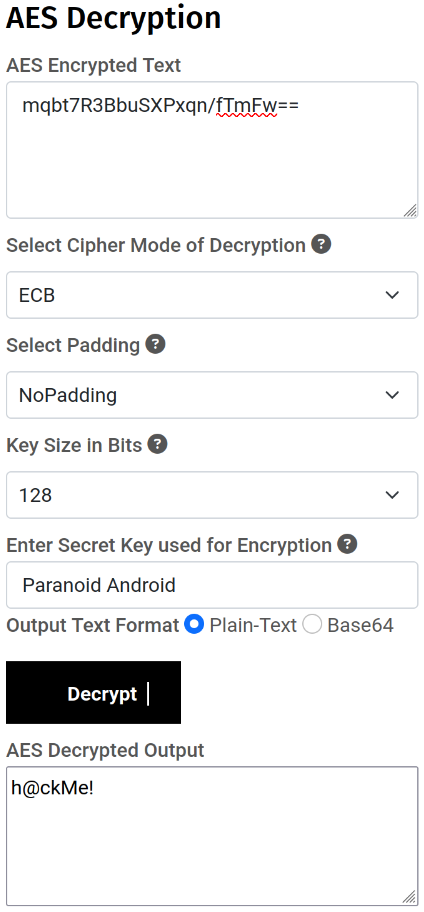
\includegraphics[width=0.4\textwidth]{aes.png}
    \caption{Decoding}
\end{figure}
\begin{figure}[H]
    \centering
    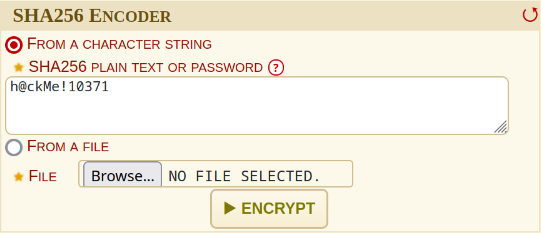
\includegraphics[width=0.5\textwidth]{encode.png}
    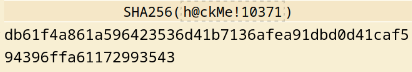
\includegraphics[width=0.5\textwidth]{hashed_password.png}
    \caption{Hashing}
\end{figure}

% End of the document
\end{document}